% this file is statistical
% will contain all final metric data

\section{Code Metrics}

\subsection{Plots of CodeMR}

\begin{figure}[H]
    \centering
    \begin{subfigure}{\textwidth}
        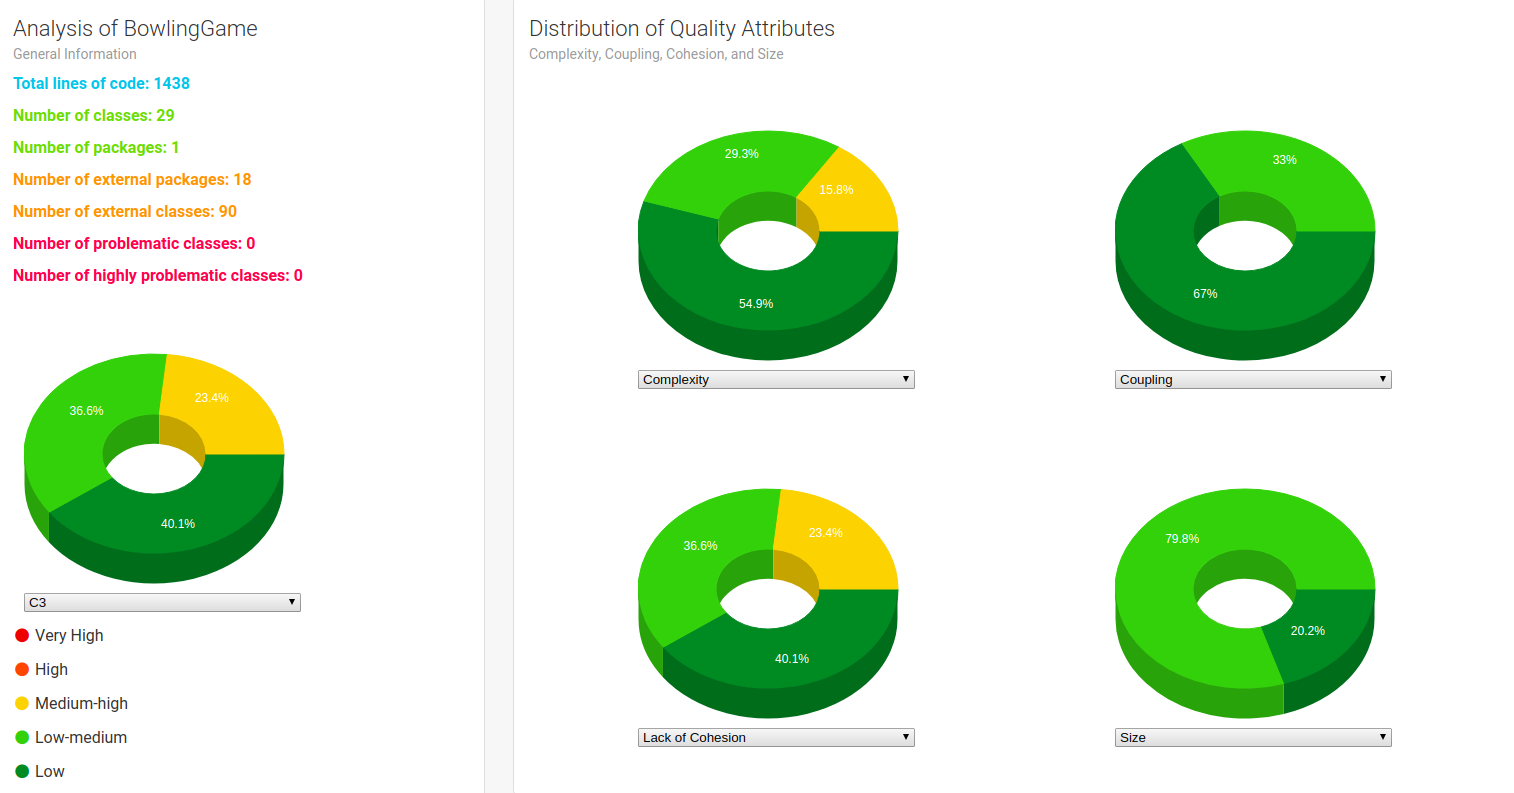
\includegraphics[width = \textwidth]{img/stats_pre.png}
        \caption{Before the Refactor}
    \end{subfigure}
    \begin{subfigure}{\textwidth}
        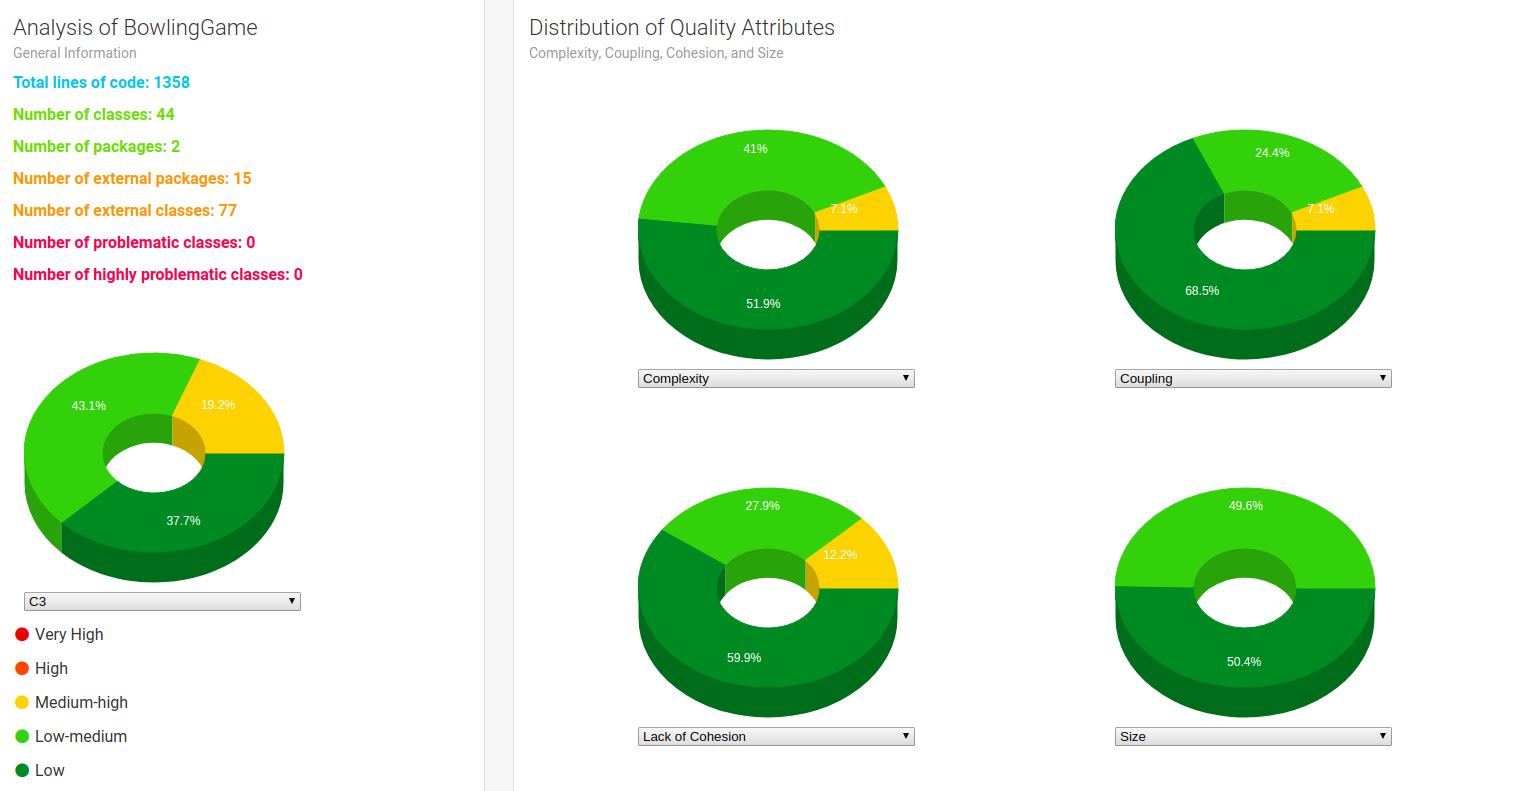
\includegraphics[width = \textwidth]{img/stats_post.png}
        \caption{After the Refactor}
    \end{subfigure}
    \caption{Code Metrics}
\end{figure}

\subsection{Metric analysis}

We investigated metrics in multiple ways: one through the CodeMR plugin for IntelliJ and the other through Metrics2 1.38 plugin for Eclipse.

\subsection{Refactoring narrative}

We present to you here the timeline of events that become the cornerstone of starting our refactoring:

\begin{itemize}

    \item Immediately, after launching metrics analyzer on the codebase, we noticed the following key components being broken: McCabe cyclomatic complexity and Nested Block Depth, with both being in Lane.java.
    \item We open Lane.java and notice it's 700 lines mammoth shape with overly complex methods. We take a guess that it's a "God class" but we're not sure.
    \item To confirm our suspicion, we look at such metrics:

          \begin{itemize}
              \item \textbf{Lack of cohesion}: it has the third highest lack of cohesion among all files.
              \item \textbf{Number of attributes}: it has the most number of attributes (18!) in a class. To be honest, 18 is a very large number and an indication that Lane.java is trying to do much.
              \item \textbf{Number of methods}: this was the killing blow. Lane.java has 17 methods, the most among all classes (the second place has only 11)
          \end{itemize}

    \item We thus concluded that Lane.java is trying to do much, and is indeed a God class.
    \item In such a system, it is ideal to start by:
          \begin{itemize}
              \item understanding all the functionality implemented in the God class
              \item marking out several sets of cohesive functionality
              \item extracting those sets out in several other classes
          \end{itemize}

    \item We then chalked out the following cohesive sets:
          \begin{itemize}
              \item Scoring functionality: \code{markScore, getScore, resetScores, isGameFinished, resetBowlerIterator}
              \item Interacting with a pinsetter: \code{getPinsetter, receivePSEvent, run}
              \item Controlling the external UI and Maintaining a observer model: \code{lanePublish, subscribe, unsubscribe, publish}
              \item Actually running the game for a party: \code{run, assignParty, isPartyAssigned}
          \end{itemize}

    \item These parts were then systematically split out into separate classes, namely, \code{ScorableParty, LaneWithPinsetter, Publisher, Lane}
    \item Once we had separate parts getting compiled, we were already ready to start ironing out complexity and redundancy issues. For quite a lot of time, we worked on these.
    \item Reducing a method for its cyclomatic complexity usually meant:
          \begin{itemize}
              \item Understanding what the method is actually doing
              \item Break it down into its core parts,
              \item Extract those core parts into new methods
              \item Reuse those new methods across the codebase
          \end{itemize}
    \item For code duplication, one thing that really stood out was the extreme disregard for redundancy in the `XView` classes, as each of them shared a series of crucial logic duplicated. For example, the logic for centering a window, or adding a button, and more. We quickly realized this and extracted out a general set of `Widget.X` classes, whose main purposes is to provide a consistent UI throughtout the codebase. This is reused throughout the codebase, and helped us creating the UI for the newer features with minimal effort.
    \item Now that we had so many classes, we ran into issues of coupling. We had to be careful when fixing those since there wasn't a general fix-all medicine for this.
    \item Once all was done, in the final stages, we made sure that cohesion scores were as high as possible. For classes that had lower cohesion, we grouped their properties and further increased cohesion.
    \item That was pretty much all :)
\end{itemize}

\subsection{Metric values analysis}

We have collected and analyzed the following key metrics, showing the before and after change in them as well.

\subsubsection{Lack of cohesion}

\textbf{Before:} 0.375 mean with 0.374 std.
\textbf{After:} 0.321 mean with 0.298 std.

This is the LCOM metric, calculated as a formula. Vales near 0 are good while near 1 are dangerous. This metric wasn't reduced significantly reduced, however, it was decently low before, so even the current scores are good.

\subsubsection{Nested block depth}
\textbf{Before:} 1.511 mean with 1.177 stdev
\textbf{After:} 1.423 mean with 0.659 stdev

Moreover, the largest offender Lane.java was brought down significantly. Top 3 before:
(Data Picked from Metrics 2)

\begin{tabular}{ |c|c|c|c| }
    \hline
    \textbf{File} & \textbf{Mean} & \textbf{Std. Dev} & \textbf{Maximum} \\
    \hline
    Lane.java     & 2.176         & 2.065             & 7                \\
    Lane.java     & 2.333         & 1.374             & 5                \\
    LaneView.java & 1.6           & 1.2               & 4                \\
    \hline
\end{tabular}

and after:

\begin{tabular}{ |c|c|c|c| }
    \hline
    \textbf{File}      & \textbf{Mean} & \textbf{Std. Dev} & \textbf{Maximum} \\
    \hline
    Lane.java          & 1.5           & 0.866             & 4                \\
    ScorableParty.java & 1.4           & 0.611             & 3                \\
    BowlerFile.java    & 2             & 0.894             & 3                \\
    \hline
\end{tabular}

\subsubsection{Instability}

\textbf{Before:} 2.319 mean with 4.062 stdev
\textbf{After:} 1.662 mean with 1.085 stdev


\subsubsection{McCabe cyclomatic complexity}

The maximum cyclomatic complexity is down significantly. These were the top four cyclomatic complexities previously:

\begin{tabular}{ |c|c|c|c| }
    \hline
    \textbf{File}       & \textbf{Mean} & \textbf{Std. Dev} & \textbf{Maximum} \\
    \hline
    Lane.java           & 5.118         & 9.498             & 38               \\
    LaneView.java       & 5.167         & 6.543             & 19               \\
    LaneStatusView.java & 3.4           & 3.878             & 11               \\
    AddPartyView.java   & 3.5           & 3.452             & 11               \\
    \hline
\end{tabular}

and these are the top four now:

\begin{tabular}{ |c|c|c|c| }
    \hline
    \textbf{File}       & \textbf{Mean} & \textbf{Std. Dev} & \textbf{Maximum} \\
    \hline
    LaneStatusView.java & 2.75          & 2.487             & 7                \\
    Lane.java           & 1.917         & 1.656             & 7                \\
    LaneView.java       & 2             & 1.414             & 5                \\
    AddPartyView.java   & 2.625         & 1.317             & 5                \\
    \hline
\end{tabular}


\subsubsection{Attribute count}

More the attributes in a class, more likely for it to be violating the Single Responsbility Principle. As is clear from the following metrics, we have ensured that such fundamental principles are not violated.


\textbf{Before:} 4.759 mean with 5.556 stdev
\textbf{After:} 2.351 mean with 2.159 stdev

The top four before:

\begin{tabular}{ |c|c| }
    \hline
    \textbf{File}      & \textbf{Count} \\
    \hline
    Lane.java          & 18             \\
    NewPatronView.java & 17             \\
    LaneView.java      & 15             \\
    AddPartyView.java  & 14             \\
    \hline
\end{tabular}

The top four now:

\begin{tabular}{ |c|c|c|c| }
    \hline
    \textbf{File}       & \textbf{Count} \\
    \hline
    LaneStatusView.java & 8              \\
    LaneEvent.java      & 7              \\
    NewPatronView.java  & 6              \\
    AddPartyView.java   & 6              \\
    \hline
\end{tabular}

\subsection{Using Metrics as a Guide}

\subsubsection{Cyclomatic Complexity}

This was an early guide which helped us simplify the methods. This in itself took apart so many coupled variables into independent segments that a lot of simplification became possible, specially by splitting lane into classes.

\subsubsection{Cohesion and Coupling}

The inheritance structure was by and large aided by the RFC & LCOM, which allowed us to split classes like Bowler into Bowler and ScorableBowler, similarly Lane into Lane and LaneWithPinsetter. Realising that there are portions of a class that use only one variable and others that use both allow this is-a type relation marking. Some places where there were parameters that only one of the methods used and not the other, we were completely able to split the classes out.

\subsection{Nesting Depth and Complexity}

Complexity was further reduced by rethinking functional logic and relizing that portions of the work can be delegated to other classes to reduce conditional nesting. This has greatly helped us delegate responsbility to the Frame and LastFrame classes, the existance of both greatly simplified nested conditionals.


\subsection{A Final View at the Scores}

All the metrics seem good. There are just 2 classes that get flagged at medium.

Lane has slightly high Complexity (RFC: 112 instead of 100), as expected, cause it's the driver, as it's the one function that calls everything else, so it's expected that there would be many method calls at some recusion depth. However, Lane is highly cohesive, and all methods are simple and semantic, making this easy to maintain. Also ScorableParty has just above normal lack of Cohesion due to the LCAM metric.

\begin{figure}[H]
    \centering
    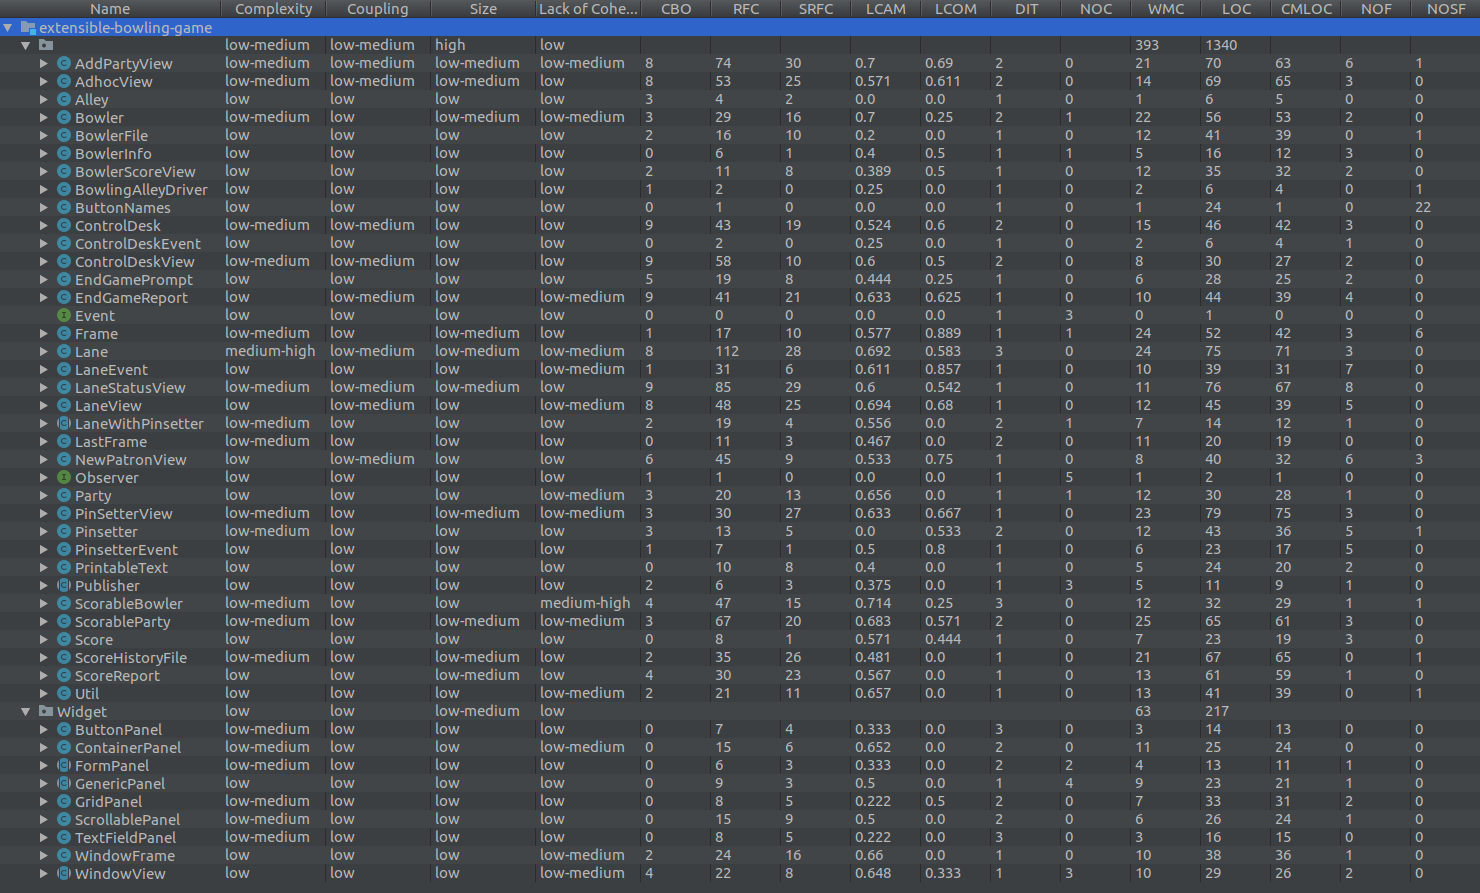
\includegraphics[width = \textwidth]{img/metric_values.png}
    \caption{Metric Values in Final Code}
\end{figure}
